\documentclass{article}

\usepackage[utf8]{inputenc}
\usepackage{xeCJK}          %导入xeCJK包
\usepackage{ctex}
\usepackage{listings}
\usepackage{xcolor}
\usepackage{graphicx}
\usepackage{float} % 导入float宏包以使用[H]参数
\usepackage{blindtext}
\usepackage{tikz}
\usepackage{algorithm}
\usepackage{algpseudocode}
\usepackage{chronology}
\usepackage{graphicx}
\usepackage{subcaption}
\usepackage{amssymb}
\usepackage{amsmath}
\usetikzlibrary{graphs, positioning, quotes, shapes.geometric}

\title{基于大语言模型的毕业设计评分系统研发}

\author{王谦益}

\date{}

\begin{document}

\maketitle

\begin{abstract}

毕业设计是每一位大学生都必须要完成的项目,对毕业设计论文的评分不仅关系着学生的毕业问题,也是评估学生写作能力、专业素质等不同方面能力的重要指标。而传统的毕业设计论文评分方式存在诸多问题,例如教师评分任务繁重、评价指标模糊、评估过程主观性强等。近年来,大语言模型(LLM)在自然语言处理领域的突破为毕业设计评分提供了新的可能性。本文介绍了一种基于大语言模型的毕业设计评分系统,该系统通过多维度评估写作内容并生成评语和建议,帮助学生改进自己的毕业设计论文,并减轻教师的评估任务。

\noindent{\textbf{关键词:}大语言模型;毕业设计评分;辅助写作;多维度评估;文本总结;少样本训练}   %加中文关键词,noindent表示缩进

\end{abstract}

\section{引言}

毕业设计论文的评分十分关键,不仅影响着学生的毕业情况,同时也是衡量学生写作素质、专业技能掌握情况的关键指标。这个评分结果能帮助学生了解自己的各方面能力综合情况,针对自身存在的问题进行针对性的改进、提升。然而传统的评分方式存在着诸多的问题。在传统评分过程当中,由于学生数量以及论文基础长度,教师的评分工作量十分巨大。随着学生人数的增加,教师需要花费大量时间进行写作批改,这增加了教师的工作负担,也影响了评估效率。\cite{ref1}其次评估标准模糊: 传统的评分方式往往缺乏明确的评估标准,导致评分结果主观性强,难以保证评分的公平性和准确性。\cite{ref2}另外评分过程反馈有限: 传统评估方式往往只提供简单的分数或评语,缺乏对学生论文内容的深入分析和指导,难以帮助学生找到改进的方向。

近年来,大语言模型(LLM)在自然语言处理领域的突破为毕业设计评分提供了新的可能性。\cite{ref2}LLM 具有强大的语言理解和生成能力,可以自动分析学生写作内容,并提供个性化的反馈和建议。因此,基于 LLM 的学生毕业设计评分系统有望解决传统评分方式的不足,提升评估效率和准确性,并为学生提供更有效的改进指导。\cite{ref3, ref4}

\section{文献调研}

在自动化作文评分(AES)领域,大型语言模型(LLMs)的应用日益受到关注。本文通过调研了一些相关论文,对目前相关领域的研究进行了整理。

首先,《Are Large Language Models Good Essay Graders?》\cite{ref7}一文较为典型。该研究直接评估了ChatGPT和Llama等LLMs在AES任务中的有效性,指出尽管LLMs展现出了一定的潜力,但它们的评分与人类评分者之间存在显著差异。特别是ChatGPT的评分往往更为严厉,与人类评分者的对齐程度较低,而Llama则表现出相对较好的一致性。此外,该论文还发现LLMs在检测拼写和语法错误方面表现出色,但这一能力并未显著提升其与人类评分者的一致性。

另一篇论文《Automatic Essay Multi-dimensional Scoring with Fine-tuning and Multiple Regression》\cite{ref8}则提出了一种创新的自动化作文多维评分系统(AEMS)。该系统通过微调和多元回归策略,实现了对作文词汇、语法、连贯性等多个维度的评分,满足了用户和学习者的多元化需求。这一研究不仅解决了传统AES系统主要提供单一整体分数的局限性,还为未来LLMs在AES领域的应用提供了新的思路。

同时综述论文《Retrieval-Augmented Generation for Large Language Models: A Survey》\cite{ref9}中提及了一项技术,“面向大型语言模型的检索增强生成” ,即RAG(Retrieval-Augmented Generation)。RAG技术通过将LLMs的内在知识与外部数据库中的广泛动态知识相结合,有效减少了生成错误内容的问题。检索阶段涉及从外部知识库中检索与查询相关的文档片段。 生成阶段将检索到的文档片段与原始查询合成为一个连贯的提示,然后输入到大型语言模型中以生成响应。增强过程通过迭代检索、递归检索和自适应检索等方法来优化RAG的性能。RAG技术通过整合参数化语言模型知识与非参数化外部数据库知识,显著增强了LLMs的能力。但同时,为了充分发挥RAG的潜力,还需要进一步研究和优化评估方法,以更准确地衡量RAG模型的性能。 

综合这几篇论文在内的其他研究不难发现,LLMs在AES任务中既具有优势也存在局限性。其优势在于强大的语言理解和生成能力,能够处理大量文本数据并提供即时反馈;而局限性则主要体现在与人类评分者之间的一致性仍有待提高。因此,未来的研究应进一步探索如何优化LLMs在AES任务中的表现,提高其与人类评分者的一致性,其中多维评分和微调策略可能将发挥重要作用。

\section{方法}

\subsection{模型结构}

\begin{figure}[H]
    \centering
    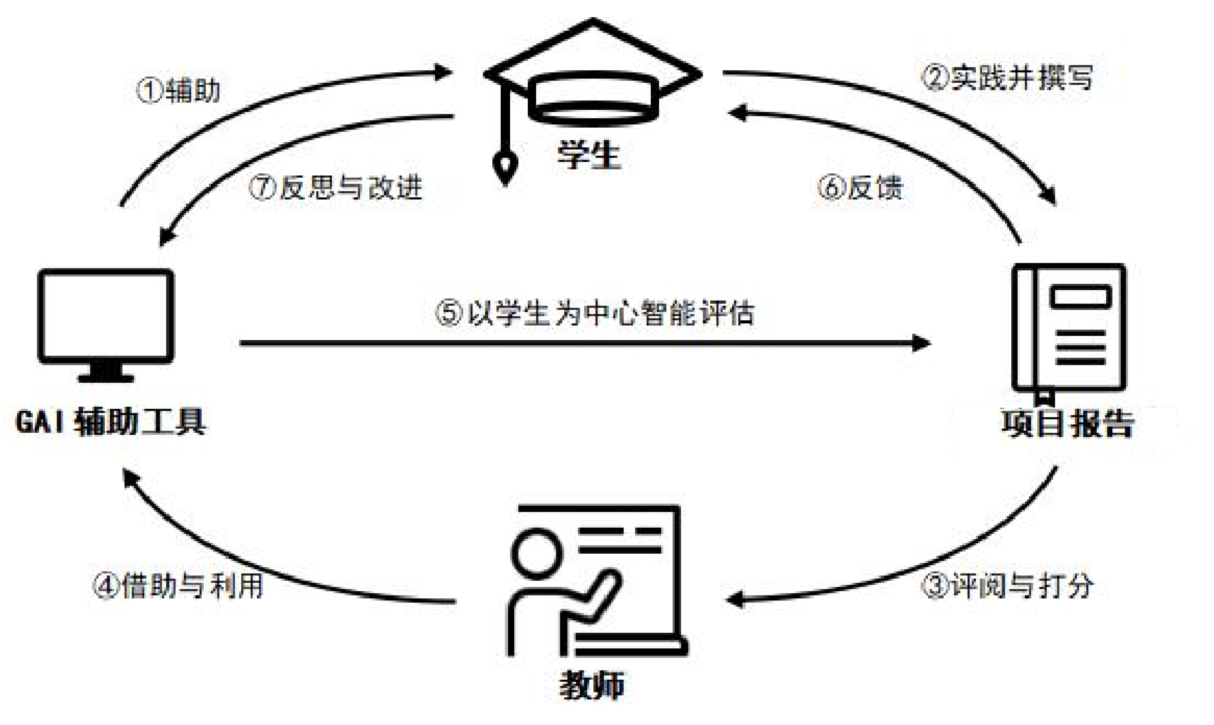
\includegraphics[width=0.75\linewidth]{img/model.png}
    \caption{GAI学生辅助系统流程}
    \label{fig:GAI}
\end{figure}

因此,一种基于大语言模型的毕业设计论文评分系统应运而生。该架构由学生、教师和由大语言模型组成的GAI辅助工具三个主要部分组成。在这套学习体系中,学生首先进行毕业设计实验以及论文撰写工作,然后接受教师的评审与打分,同时教师也利用GAI辅助工具为学生的论文进行打分和评价,最后教师会综合自身和GAI工具的得分给出最终评估结果。学生会从最终结果中收到的反馈进行反思和改进,以修正自己毕业设计中的缺点与不足之处。其中GAI辅助工具不仅能辅助教师完成打分任务,还可以为学生提供各种形式的帮助和服务,如文本分析、语法检查、词汇推荐等,从而帮助学生更好地完成论文撰写工作、提高论文质量。这种基于大语言模型的智能评分系统能够有效地整合各方资源和技术优势,为学生们提供一个全面且高效的学习平台,帮助他们不断提升自身的综合素质和能力水平。

\subsection{多维度评估方法}

在评估毕业设计论文的时候,没法直接让大语言模型输出理想的结果,而需要为大语言模型提供一套合理的评估方案和打分标准。目标是希望提供的评分方案能够得到细化且全面的毕业设计论文评估报告,以给出综合且客观的评价。多维度的评估方法是一种综合性的评价方式,它通过对多个维度的考量来全面地衡量某一对象或现象的特征和价值。因此提出多维度评估方法来实现目标,其中包括以下几个方面:1.结构完整,评估对象的总体框架是否严谨,内部布局是否合理。这要求评估者具备一定的专业知识和经验,能够从整体上把握事物的内在逻辑关系和外在表现形式;2.逻辑清晰,考察论证过程的条理性和连贯性,看其是否能准确表达观点、论据和结论之间的关系,并且是否存在明显的漏洞或不一致之处;3.语言流畅,关注的是语言的运用是否恰当得体,句子结构是否符合语法规范,避免因语病而导致误解的情况发生。4.内容是否独特与创新,强调所呈现的内容是否有新意或有独到见解,能否引起读者的兴趣或启发思考。此外还需要对参考文献规范性进行检查,检查引用文献的格式是否符合学术界的通用标准,确保信息的来源可靠且可追溯;以及有必要通过报告了解学生对于相关课程的知识的理解和应用程度,了解他们是否真正掌握了所学内容并能灵活运用在实际工作中。

因此总共设计了6个维度的评估标准,其中前四个维度(结构完整性、逻辑清晰度、语言流畅性、内容独特与创新性)作为评估报告的主要维度,而参考文献和课程内容理解我们将其作为次要维度,在评分中占比较小。

\subsection{提示词}

好的大模型反馈离不开好的提示词的设计。\cite{ref5}为了让大模型反馈出更加符合需求的内容,需要设计提示词对大模型提出需求。在为学生毕业设计论文的模型中,提示语需要为大模型加入加入语境背景或角色,通过提示词让大模型理解它所处理的事务和扮演的角色;其次提示语还需要进行词汇解释,确保提示词中的关键术语和概念清晰明确;为了确保标准化的输出,提示词中还需要额外添加模板输出或占位符,为模型生成的内容提供结构和框架;最后调整和优化提示词,以控制模型生成的输出内容,避免冗余或偏离主题。\cite{ref6}经过设计后的提示词如下图:

\begin{figure}[H]
    \centering
    
\includegraphics[width=0.75\linewidth]{img/prompt.png}
    \caption{提示词设计}
    \label{fig:prompt}
\end{figure}

\subsection{系统交互模块}

\begin{figure}[H]
    \centering
    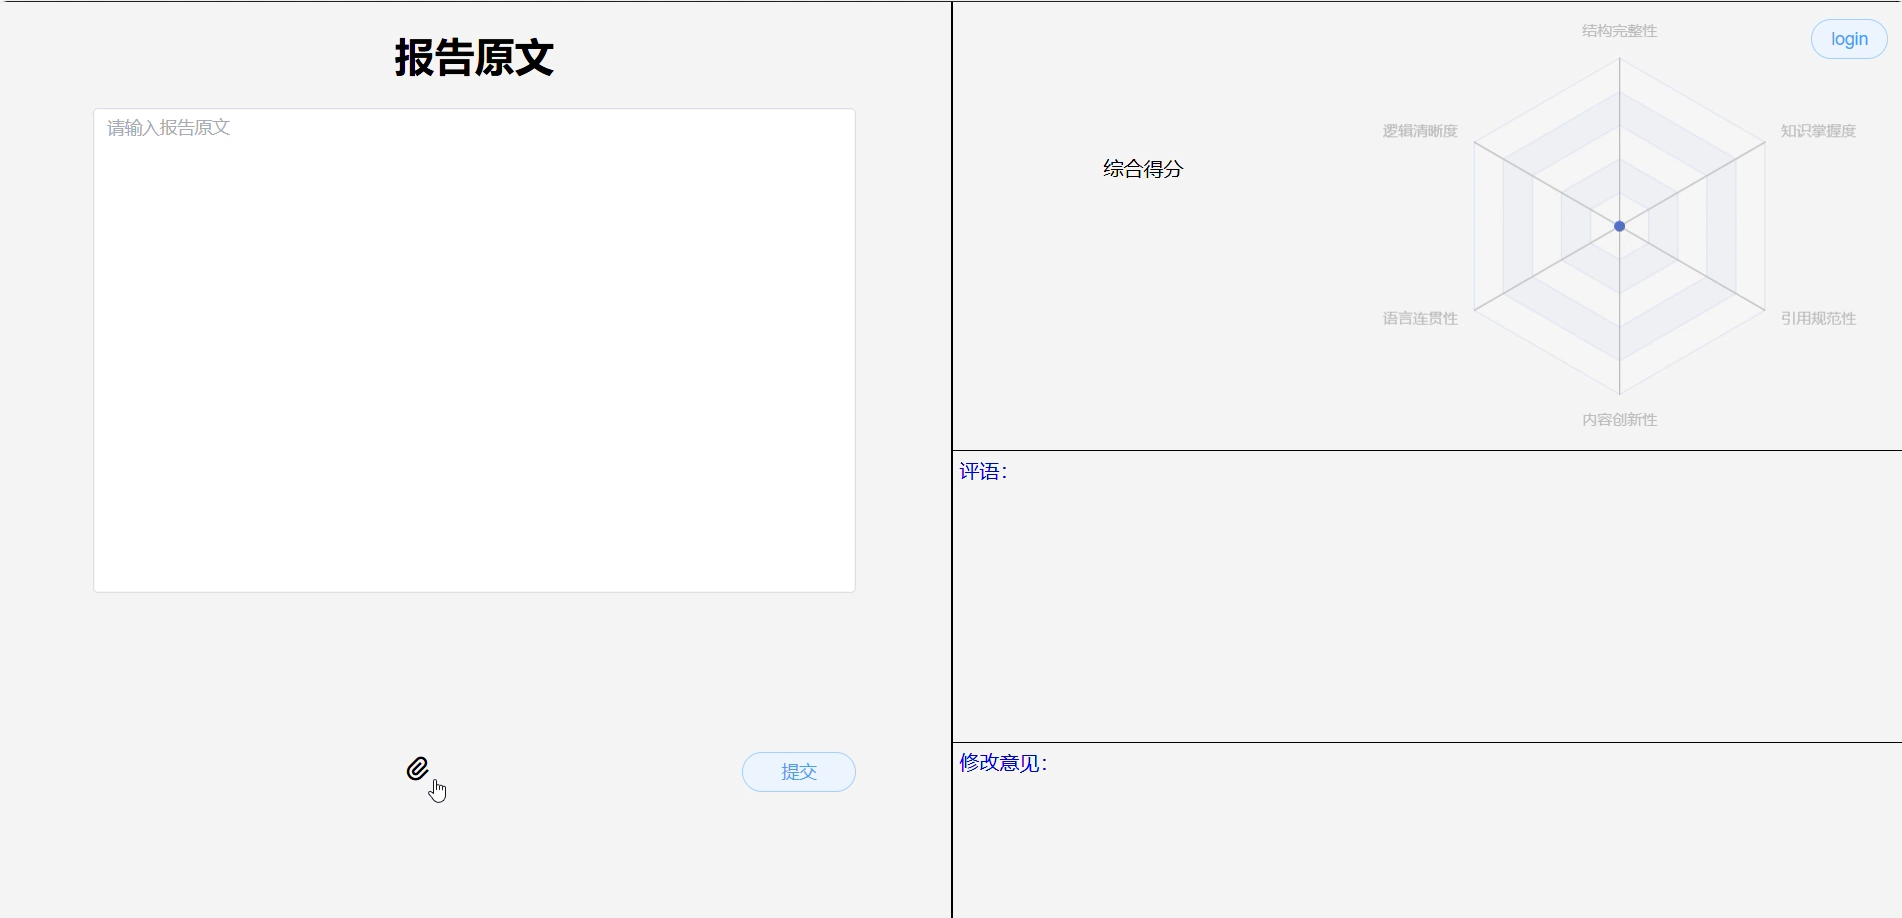
\includegraphics[width=0.9\linewidth]{img/frontEnd.png}
    \caption{系统交互界面}
    \label{fig:frontEnd}
\end{figure}

为了方便可视化操作,设计系统交互界面是必不可缺的步骤。从图3中可以看到前端提供了一个直观的用户界面,用于连接大型语言模型(LLM)与学生毕业设计论文评分功能。界面的左侧区域专门用于输入待评估的报告原文,同时也可以直接传入文本文件。传入后大模型会根据预设好的提示词对文本内容进行分析。右侧则显示了综合评分以及多维度的详细评估结果。

\section{实验}

\subsection{实验准备}

\subsubsection{数据集}

\begin{figure}[h!]
	\centering
	\begin{subfigure}{0.45\linewidth}
		\centering
		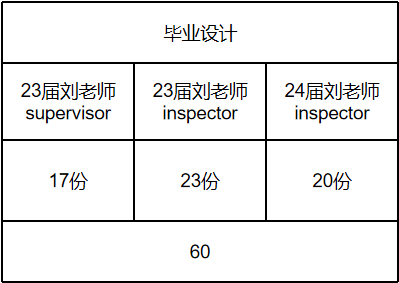
\includegraphics[width=0.9\linewidth]{img/data-consistent.png}
		\caption{数据组成}
		\label{fig:data-consistent}
	\end{subfigure}
	\centering
	\begin{subfigure}{0.45\linewidth}
		\centering
		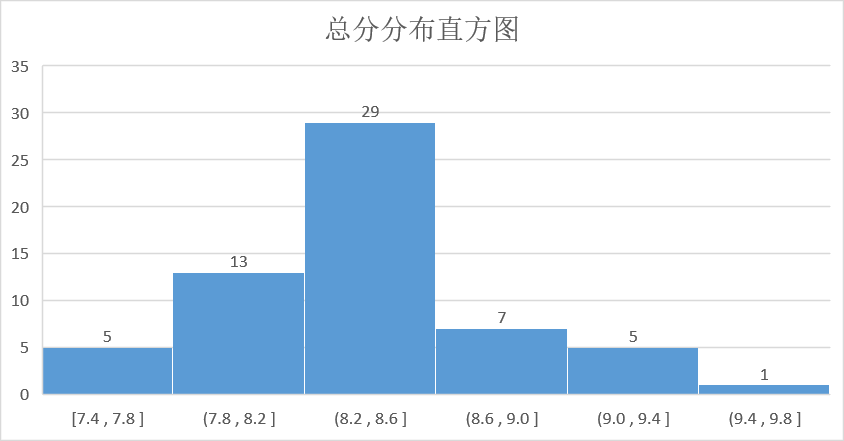
\includegraphics[width=0.9\linewidth]{img/data-graph.png}
		\caption{数据直方图}
		\label{fig:data-graph}
	\end{subfigure}
    \centering
	\begin{subfigure}{0.9\linewidth}
		\centering
		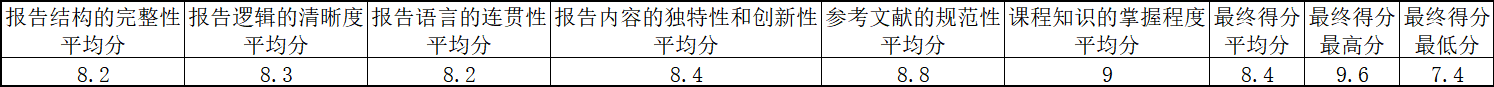
\includegraphics[width=0.9\linewidth]{img/data-average.png}
		\caption{数据统计}
		\label{fig:data-average}
	\end{subfigure}
	\caption{数据集}
		\label{fig:dataset}
\end{figure}

实验当中使用的数据集来自课题组收集的2023、2024年计算机系本科生毕业设计论文。数据集包含不同年级、不同课题的毕业设计报告。每篇报告都有教师人工打分,较有利于我们后续对比模型结果和对作者相关属性进行分析。

\subsubsection{数据清洗}

毕业设计论文均为PDF格式,但是其中会包含很多不同类型的数据,包括但不限于文字、图片、表格等。因此需要使用工具包(例如PyPDF2)对报告进行文字提取,并在之后进行人工审核校对,纠正对于PDF文件页面分栏识别的问题。为保证结构完整性、参考文献规范性等评分维度不受人为因素影响,尚未对提取出的纯文本数据进行格式上的规整,还保留脚本提取后的分段、换行等格式。

\subsection{多维度评估+提示词}

\subsubsection{网页端大模型初尝试}

首先使用设计好的提示词,对目前开源的大语言模型进行测试。其中,模型选择了:文心一言、通义千问、deepseek以及chatGPT,这三个国内模型一个国外模型。使用的数据是2023本科论文的其中5篇进行了简单的测试,所有维度和总分的设计是0之10分,4个主要维度各占比系数0.2,次要维度各占比系数0.1。取所有维度和总分的平均得分进行分析。

\begin{figure}
    \centering
    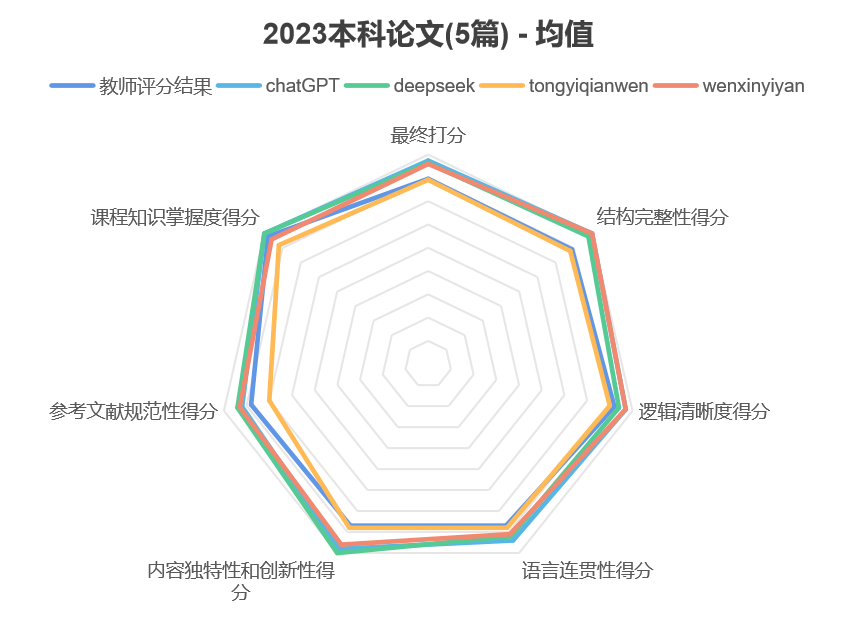
\includegraphics[width=0.5\linewidth]{img/2023(5)-webui-average.png}
    \caption{2023本科论文(5篇) - 均值}
    \label{fig:webui-2023(5)-average}
\end{figure}

对比教师的人工打分,不难发现通义千问的打分结果与教师标准最接近。 通义千问在结构完整性、逻辑清晰度等核心指标上与教师评分高度一致,尤其在参考文献规范性(7.0 vs 教师7.8)和内容创新性(7.8 vs 教师7.7)上表现贴近。而其他模型(如ChatGPT、DeepSeek)在创新性、语言连贯性等维度显著高于教师评分,可能存在“过拟合”或评分宽松的问题。 

\begin{figure}[h!]
	\centering
	\begin{subfigure}{0.3\linewidth}
		\centering
		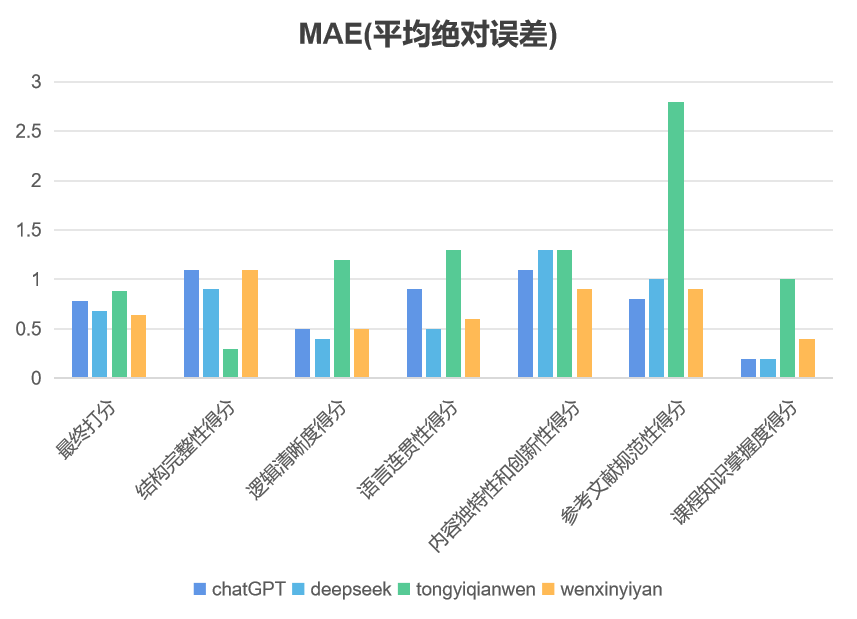
\includegraphics[width=0.9\linewidth]{img/2023(5)-webui-MAE.png}
		\caption{2023本科论文(5篇) - MAE(平均绝对误差)}
		\label{fig:webui-2023(5)-MAE}
	\end{subfigure}
	\centering
	\begin{subfigure}{0.3\linewidth}
		\centering
		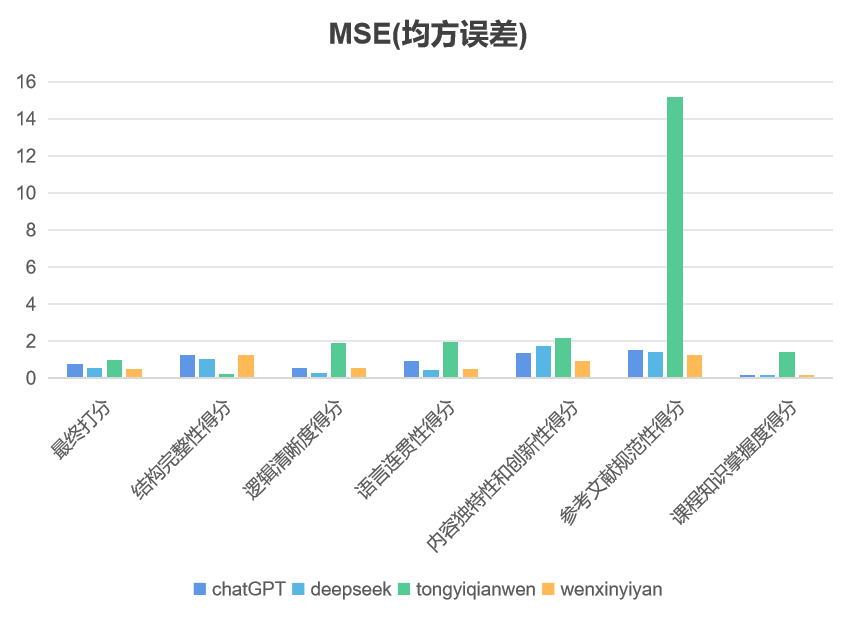
\includegraphics[width=0.9\linewidth]{img/2023(5)-webui-MSE.png}
		\caption{2023本科论文(5篇) - MSE(均方误差)}
		\label{fig:webui-2023(5)-MSE}
	\end{subfigure}
    \centering
	\begin{subfigure}{0.3\linewidth}
		\centering
		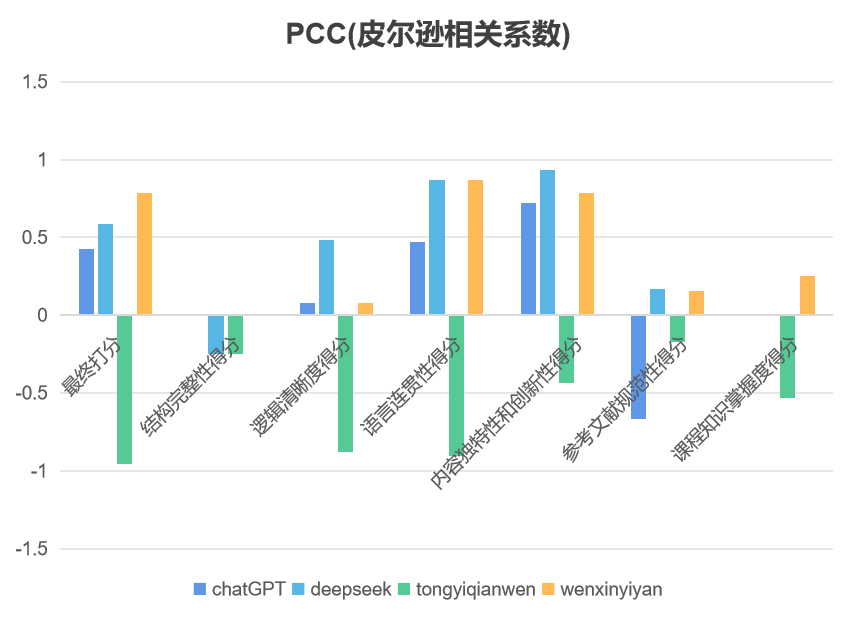
\includegraphics[width=0.9\linewidth]{img/2023(5)-webui-PCC.png}
		\caption{2023本科论文(5篇) - PCC(皮尔逊相关系数)}
		\label{fig:webui-2023(5)-PCC}
	\end{subfigure}
	\caption{2023本科论文(5篇) - metrics}
		\label{fig:webui-2023(5)-metrics}
\end{figure}

根据MSE、MAE和PCC三项指标的综合分析,文心一言在贴合教师评分标准方面表现最优,其MSE最低(0.488)、MAE较小(0.64),且PCC最高(0.78),表明其评分偏差最小且与教师标准高度正相关。DeepSeek紧随其后,MSE(0.576)和MAE(0.68)较低,PCC(0.59)显示其逻辑清晰度和语言连贯性与教师评分较为接近,但在内容创新性上存在一定偏差。ChatGPT表现中等,MSE(0.75)和MAE(0.78)略高,PCC(0.42)显示其相关性一般,尤其在创新性评分上与教师标准差异较大。通义千问则显著偏离教师标准,MSE(1.004)和MAE(0.88)均为最高,PCC(-0.95)呈现极端负相关,尤其在参考文献规范性(MSE=15.2)和逻辑清晰度(PCC=-0.88)上表现异常。

总体来看,文心一言是最贴合教师评分结果的模型,假设允许一定程度的灵活性,则可结合DeepSeek和ChatGPT的优势;而通义千问因多项指标偏离较大则不太适合。

 \subsubsection{百炼平台模型实验}

上述结果只用了5篇数据,结果并没有很强的说服性,因此后续为了通过大量数据取得稳定结果,利用了阿里云百炼平台上的多种模型接口进行了进一步实验。其中,实验选择的模型包括:通义千问-Plus、通义千问2.5-14B-1M、通义千问-Turbo、DeepSeek-V3、DeepSeek-R1。这次实验当中使用的数据全部60篇毕业设计论文,所有维度和总分的设计依旧是0之10分,各个维度数据占比不变。

\begin{figure}
    \centering
    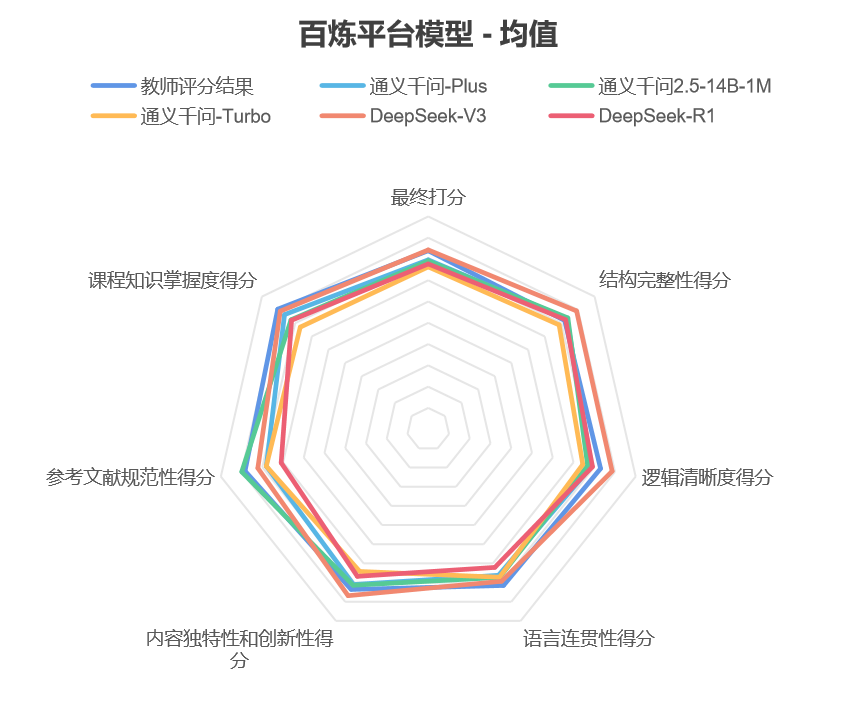
\includegraphics[width=0.5\linewidth]{img/bailian-average.png}
    \caption{百炼 - 均值}
    \label{fig:bailian-average}
\end{figure}

为了评估哪个模型更贴合教师评分标准,引入了欧氏距离(Euclidean Distance)作为衡量标准,计算每个模型与教师评分在各维度上的差异。 

\[Distance=\sqrt{\sum_{i=1}^{n} ​(Ti​−Mi​)^{2}}\]
其中,$T_{i}$ 是教师评分,$M_{i}$ 是模型评分。 结果如下:

\begin{table}
    \centering
    \begin{tabular}{cc}
         模型& 欧氏距离\\
         DeepSeek-V3& 0.908\\
         通义千问-Plus& 1.072\\
         通义千问2.5-14B-1M& 1.169\\
         DeepSeek-R1& 1.431\\
         通义千问-Turbo& 1.843\\
    \end{tabular}
    \caption{百炼-均值-欧氏距离}
    \label{tab:bailian-average-EuclideanDistance}
\end{table}

DeepSeek-V3 的欧氏距离最小(0.908),说明它在各评分维度上最接近教师评分标准,是表现最好的模型。其次是通义千问-Plus(1.072)和通义千问2.5-14B-1M(1.169)。 

\begin{figure}[h!]
	\centering
	\begin{subfigure}{0.3\linewidth}
		\centering
		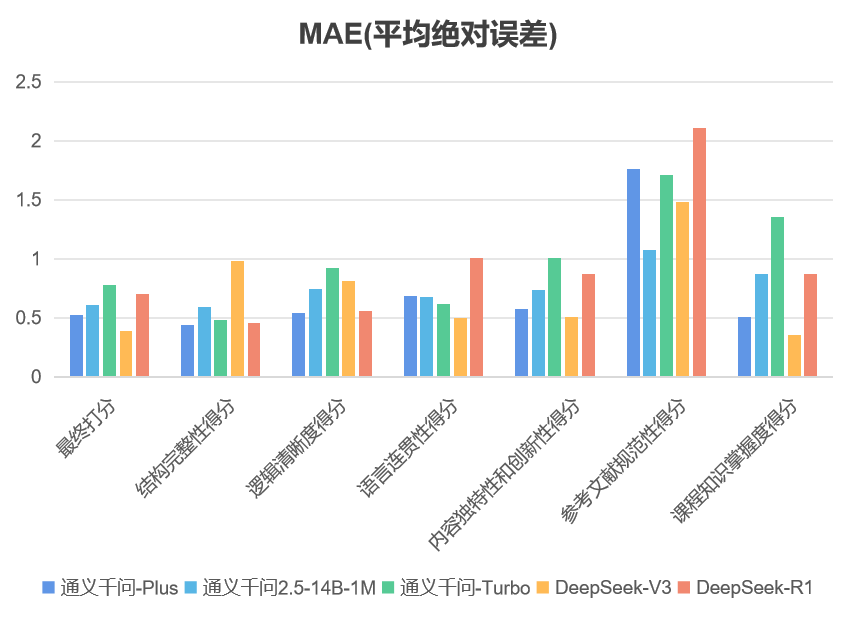
\includegraphics[width=0.9\linewidth]{img/bailian-MAE.png}
		\caption{百炼 - MAE(平均绝对误差)}
		\label{fig:bailian-MAE}
	\end{subfigure}
	\centering
	\begin{subfigure}{0.3\linewidth}
		\centering
		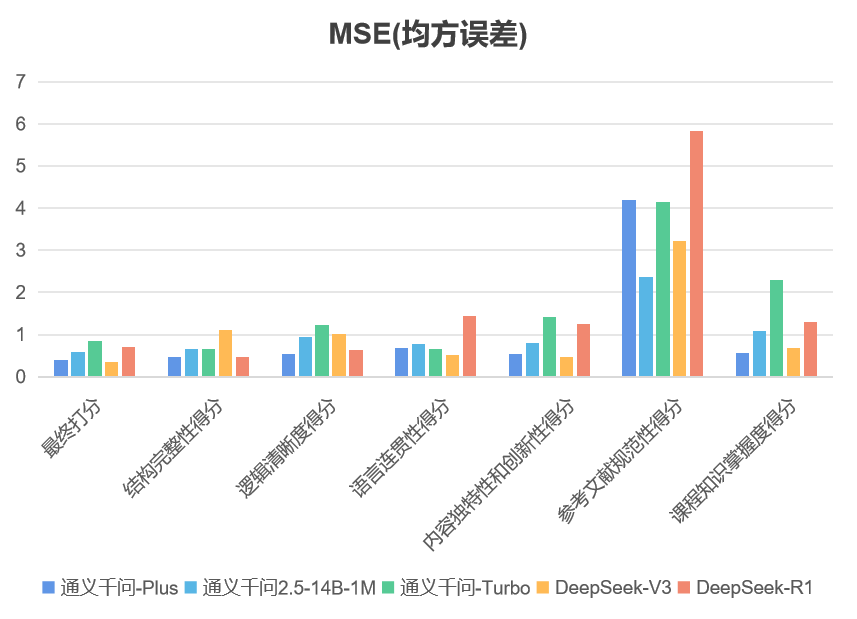
\includegraphics[width=0.9\linewidth]{img/bailian-MSE.png}
		\caption{百炼 - MSE(均方误差)}
		\label{fig:bailian-MSE}
	\end{subfigure}
    \centering
	\begin{subfigure}{0.3\linewidth}
		\centering
		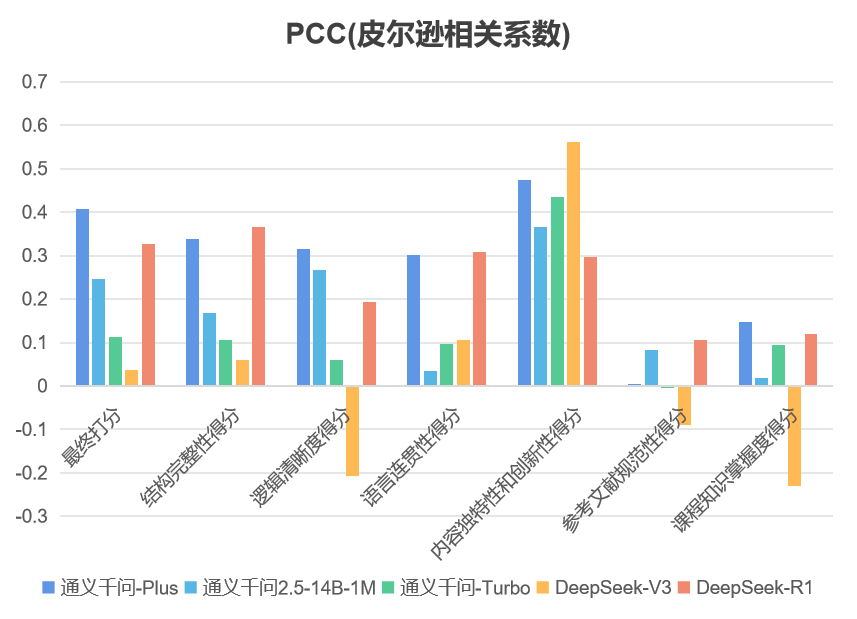
\includegraphics[width=0.9\linewidth]{img/bailian-PCC.png}
		\caption{百炼 - PCC(皮尔逊相关系数)}
		\label{fig:bailian-PCC}
	\end{subfigure}
	\caption{百炼 - metrics}
		\label{fig:bailian-metrics}
\end{figure}

从MSE、MAE和PCC三个指标的综合分析来看,DeepSeek-V3在整体评分上最贴合教师标准,其最终打分的MSE(0.358)和MAE(0.39)均为最低,表明其评分误差最小,稳定性最佳。不过,其PCC(0.036)接近0,说明评分趋势与教师标准相关性较弱,可能更适合需要保守评分的场景。通义千问-Plus在结构完整性(MAE=0.442)和逻辑清晰度(MAE=0.542)上表现突出,PCC(0.406)也是各模型中最高的,显示出较好的评分趋势一致性,适合注重论文结构与逻辑严谨性的需求。此外,通义千问2.5-14B-1M在参考文献规范性(MSE=2.363)上优于其他版本,适合需要规范引用的学术写作。然而,各模型在参考文献规范性上的表现普遍较差,仍有优化空间。综合来看,若以最小化误差为目标,DeepSeek-V3是最佳选择;若需兼顾结构与逻辑的准确性,通义千问-Plus更为合适。未来改进可重点关注提升参考文献规范性和评分趋势的一致性。 

\subsection{少样本模型微调}

在深入对比了包括阿里云百炼平台、百度千帆平台、智普平台等多个主流开源模型平台之后发现,尽管这些平台提供了高效的文本生成和评分功能,但它们生成的评分结果与教师的人工评分结果之间依然存在明显差距。具体而言,模型所生成的评分及评语在准确性、一致性以及细节层面,未能完全符合教师的评分标准。因此,为了更好地契合实际需求,并缩小模型与人工评分之间的差距,需要基于现有的开源大模型,通过少样本训练的方式,针对性地对模型进行精调,以提高其在特定任务中的表现。

\subsubsection{数据处理}

\begin{figure}
    \centering
    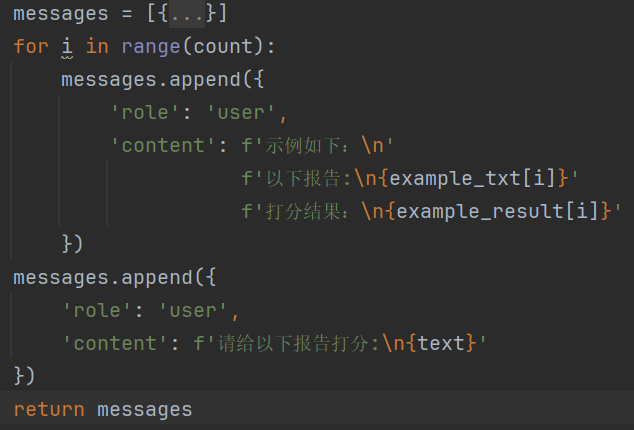
\includegraphics[width=1\linewidth]{img/few-shot.png}
    \caption{提示语微调}
    \label{fig:few-shot}
\end{figure}

选用2024本科论文中的5篇论文,提取文字内容以及教师打分结果,分别存储在\texttt{\textit{example\_txt}}和\texttt{\textit{example\_result}};两个列表当中。随后通过prompt将其依次添加到模型输入信息当中,进行少样本学习来微调模型。由于平台模型输入长度限制,最后只能选取3篇报告进行实验。


\subsubsection{精调结果与分析}

\begin{figure}
    \centering
    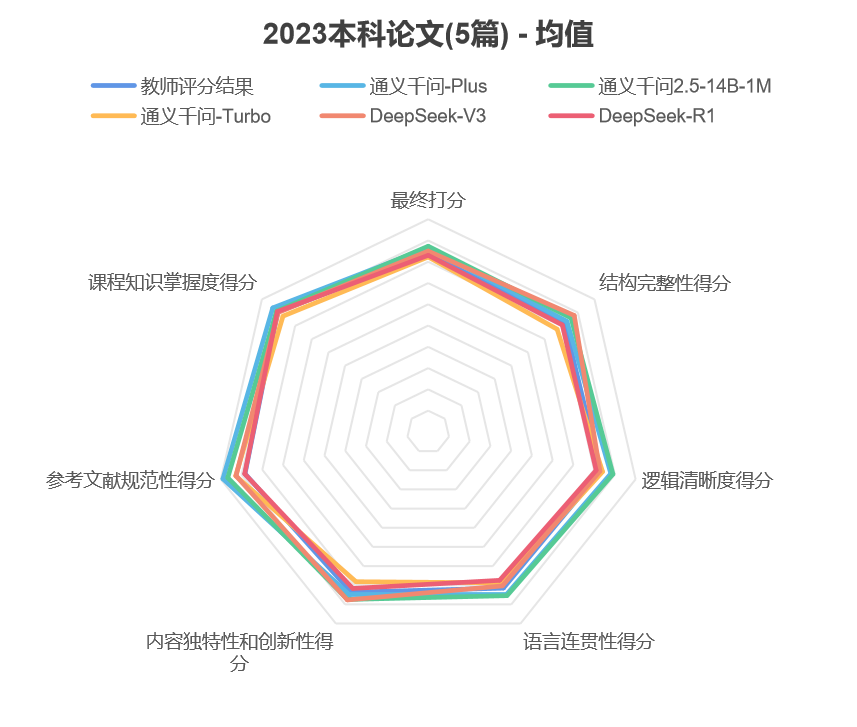
\includegraphics[width=0.5\linewidth]{img/bailian-fewShot3-average.png}
    \caption{百炼 - few-shot=3 - 均值}
    \label{fig:bailian-fewShot3-average}
\end{figure}

DeepSeek-V3和通义千问2.5-14B-1M在贴合教师评分标准方面表现突出。改进后的模型中,DeepSeek-V3在贴合教师评分标准上表现最为均衡,其核心优势体现在与教师评分高度契合的课程知识掌握度(9.02 vs 教师9.05)和逻辑清晰度(8.28 vs 教师8.31),总分差距仅0.113分,且通过内容创新性(+0.41)和参考文献规范性(+1.05)的稳健提升实现了均衡优化。通义千问2.5-14B-1M虽以总分8.732位列第一,但逻辑清晰度(8.91)、结构完整性(8.59)等多项指标显著高于教师标准,存在过度优化风险,更适合强调创新性(8.74)和文献规范(9.67)的场景。通义千问-Plus和DeepSeek-R1分别通过局部强化参考文献规范性(+2.092)和课程知识贴合度(9.08)取得进步,但存在语言连贯性(7.74)或逻辑偏离(8.91)的短板。

\begin{figure}[h!]
	\centering
	\begin{subfigure}{0.3\linewidth}
		\centering
		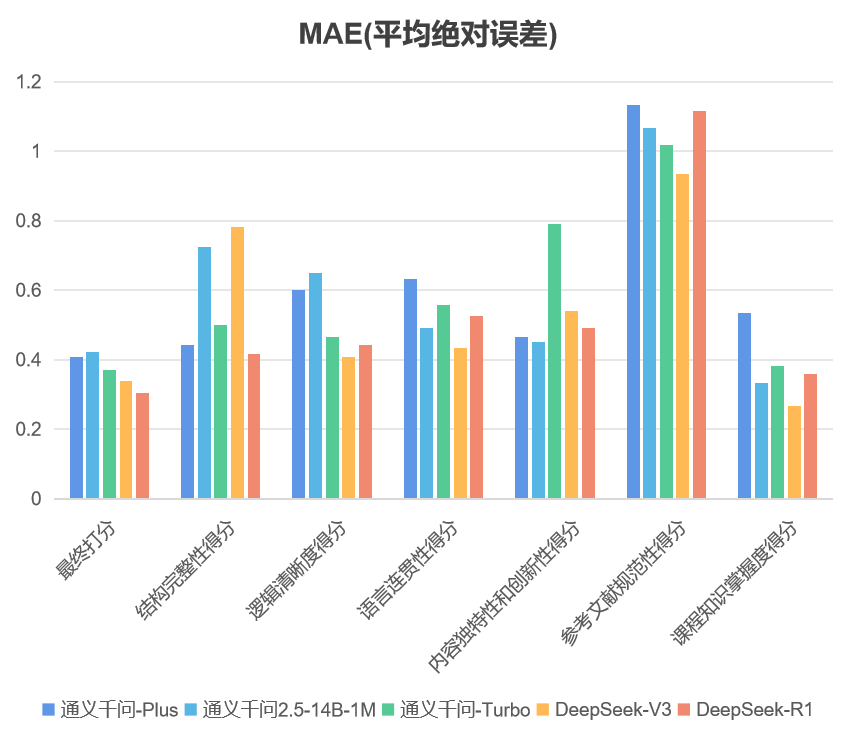
\includegraphics[width=0.9\linewidth]{img/bailian-fewShot3-MAE.png}
		\caption{百炼 - few-shot=3 - MAE(平均绝对误差)}
		\label{fig:bailian-fewShot3-MAE}
	\end{subfigure}
	\centering
	\begin{subfigure}{0.3\linewidth}
		\centering
		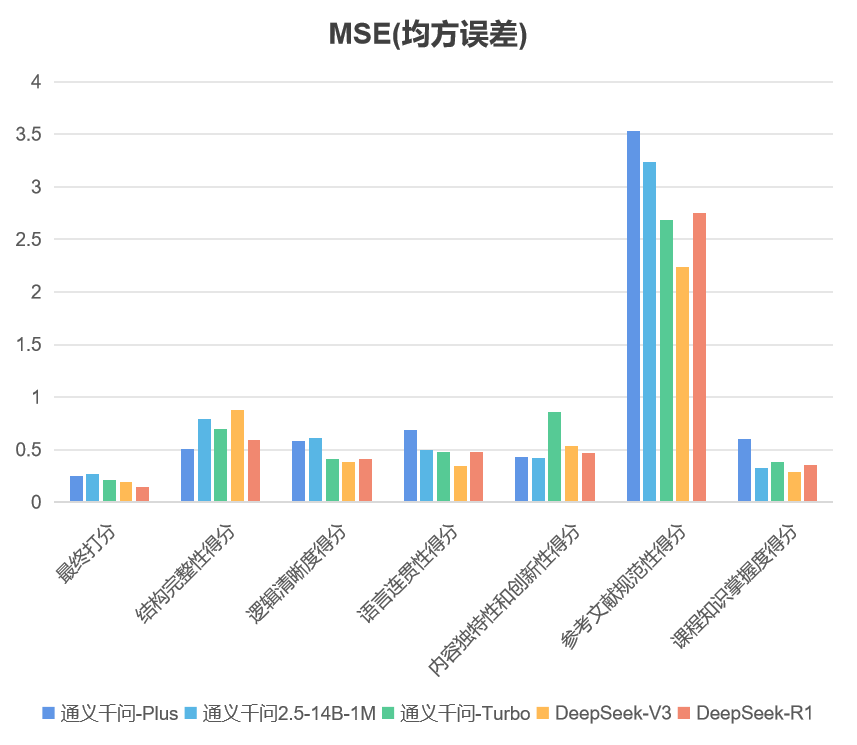
\includegraphics[width=0.9\linewidth]{img/bailian-fewShot3-MSE.png}
		\caption{百炼 - few-shot=3 - MSE(均方误差)}
		\label{fig:bailian-fewShot3-MSE}
	\end{subfigure}
    \centering
	\begin{subfigure}{0.3\linewidth}
		\centering
		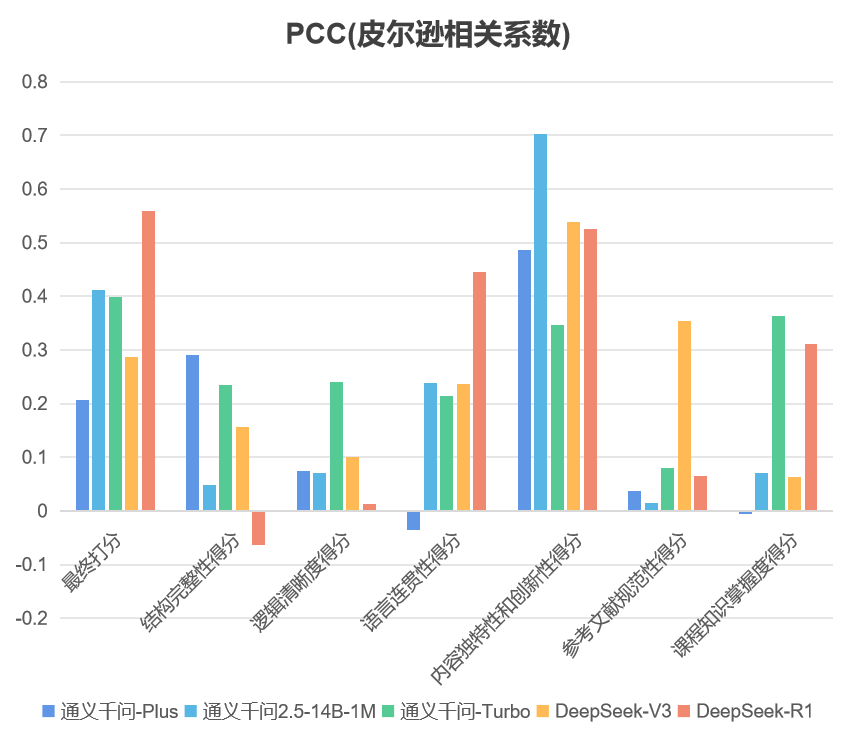
\includegraphics[width=0.9\linewidth]{img/bailian-fewShot3-PCC.png}
		\caption{百炼 - few-shot=3 - PCC(皮尔逊相关系数)}
		\label{fig:bailian-fewShot3-PCC}
	\end{subfigure}
	\caption{百炼 - few-shot=3 - metrics}
		\label{fig:bailian-fewShot3-metrics}
\end{figure}

各模型在贴合教师评分标准上的表现显著优化。DeepSeek-R1成为最接近教师打分的模型,其最终打分的MSE(0.148)和MAE(0.303)均降至最低,且PCC(0.558)跃居首位,尤其内容创新性评分(PCC=0.525)与教师标准高度契合;DeepSeek-V3则保持低误差优势(MSE=0.19),同时参考文献规范性大幅提升(PCC从-0.091升至0.355)。

通义千问系列中,Turbo版本改进最为显著,最终打分误差降低75.5\%(MSE=0.207),但内容创新性误差仍偏高(MSE=0.854);Plus版本在结构完整性(MAE=0.442)和语言连贯性上维持优势,但参考文献规范性(MSE=3.533)仍是短板。

改进后,若需平衡精度与趋势,DeepSeek-R1为最优选择;重视引文规范可选DeepSeek-V3;而通义千问2.5-14B凭借内容创新性趋势贴合度(PCC=0.702)适合学术创新评估。当前共性问题是参考文献规范性和部分指标趋势相关性,如DeepSeek-R1结构完整性PCC=-0.064),需进一步针对性优化。 

总的来说,本次精调训练成功提升了模型的评分效果,为后续的模型优化和实际应用打下了坚实的基础。未来将在更多数据和更强模型的支持下,进一步改善现有结果,并实现更加精准的自动评分系统。

\section{总结}

本文介绍了一种基于大语言模型的毕业设计论文智能评分系统。其中提出了利用GAI辅助工具提升教师评价和学生毕业设计论文质量的系统架构,并通过多维度评估设计大模型的提示词进行实验测试。通过设计合适的提示词,大语言模型能够根据这些维度对写作内容进行分析,并生成综合评分和详细的评估结果,但直接将原文输入给大语言模型打分的结果和教师打分有一定差距。为了优化模型对文本的理解和打分效果,尝试使用少样本模型微调的方式。实验结果表明,精调后的模型在评分一致性和准确性上得到了显著提升。

未来将借鉴RAG技术,通过检索增强以及模型微调相结合等方式继续改进系统,提升评估效果。计划进一步完善评估标准,使其更加全面和准确,并能够评估学生的写作风格、情感表达等方面。此外还可以分析具体得分和学生属性的相关性,提供更详细的评估结果解释,帮助学生理解评估结果,并进行针对性的改进。并且还会进一步完善网页系统,使其能够支持多文件并发请求,同时添加自定义提示词等其他功能设计。

\begin{thebibliography}{99}

\bibitem{ref1}翟洁,李艳豪,李彬彬,等.基于大语言模型的个性化实验报告评语自动生成与应用[J/OL].计算机工程,1-10[2024-11-09].https://doi.org/10.19678/j.issn.1000-3428.00EC0069593.

\bibitem{ref2}薛嗣媛,周建设. 大语言模型在汉语写作智能评估中的应用研究[J]. 昆明学院学报,2024,46(2):10-22. DOI:10.14091/j.cnki.kmxyxb.2024.02.002.

\bibitem{ref3}Link, S., Mehrzad, M., \& Rahimi, M. (2022). Impact of automated writing evaluation on teacher feedback, student revision, and writing improvement. Computer Assisted Language Learning, 35(4), 605-634. doi:https://doi.org/10.1080/09588221.2020.1743323

\bibitem{ref4}Pankiewicz, M., \& Baker, R. S. (2023). Large language models (GPT) for automating feedback on programming assignments. Ithaca: Retrieved from https://www.proquest.com/working-papers/large-language-models-gpt-automating-feedback-on/docview/2832896659/se-2 

\bibitem{ref5}A. Ramprasad and P. Sivakumar, "Context-Aware Summarization for PDF Documents using Large Language Models," 2024 International Conference on Expert Clouds and Applications (ICOECA), Bengaluru, India, 2024, pp. 186-191, doi: 10.1109/ICOECA62351.2024.00044. 

\bibitem{ref6}White, J., Fu, Q., Hays, S., Sandborn, M., Olea, C., Gilbert, H., . . . Schmidt, D. C. (2023). A prompt pattern catalog to enhance prompt engineering with ChatGPT.Ithaca: Retrieved from https://www.proquest.com/working-papers/prompt-pattern-catalog-enhance-engineering-with/docview/2779271809/se-2

\bibitem{ref7}arXiv:2409.13120

\bibitem{ref8}arXiv:2406.01198

\bibitem{ref9}arXiv:2312.10997

\end{thebibliography}


\end{document}
